\chapter{Spatial Transformations for the Computations of the Log-composition: SE(2) and Diff}\label{ch:spatial_transformations}


\begin{flushright}
	\emph{Every working mathematician knows that if one does not control oneself (best of all by examples), then after some ten pages half of all the signs in formulae will be wrong and twos will find their way from denominators into numerators. \\ -V.I. Arnold}
\end{flushright}

\noindent
In the previous chapter we have introduced some essential mathematical tools for the numerical computation of the log-composition. Each of the theoretical elements depends strongly on the transformations considered, and in this chapter we will see how they can be applied for the cases of $SE(2)$ and the for the Lie group of diffeomorphisms parametrized with stationary velocity fields:
\begin{enumerate}
	\item[$SE(2)$ -] The group of rigid body transformation of the plane (any combination of bi-dimensional rotations and translations) is a good playground to test the numerical methods introduced so far, since results can be compared with a closed form.
	A representation of this Lie group as a subgroup of the general linear group $GL(2)$, with corresponding Lie algebra will be provided, with closed form for the log-computation.
	\item[$\text{Diff}(\Omega)$ -] The group of diffeomorphisms over $\Omega$, indcated with $\text{Diff}(\Omega)$ is defined over the wide set of all of the differentiable and invertible functions. For our applications we will restrict the set to the diffeomorphisms that can be parametrized by stationary velocity fields or SVF. This set, indicated with $\Gamma$ has remarkable property thanks to the one-parameter subgroup, and its elements are in correspondence with SVF that belongs to the Lie algebra of $\text{Diff}(\Omega)$. The infinite dimensional vector space of stationary velocity field, is the second group utilized to test the numerical methods here presented for the computation of the log-composition. In this case we do not know any closed form, but considering an \lq\lq improper norm\rq\rq~ in the space of deformations it is possible to compare SVF and assess the quality of the results.
\end{enumerate}


\section{The Lie Group of Rigid Body Transformations}\label{se:rigid_body_transformations}
% group
Each element of the group of rigid body transformation (or euclidean group) $SE(2)$ can be computed as the consecutive application of a rotation and a translation applied to any point $(x,y)^T$ of the plane:
\begin{align*}
\left (  
\begin{array} {c }
X \\
Y
\end{array}
\right )  
= 
R(\theta)
\left (  
\begin{array} {c }
x \\
y
\end{array}
\right ) 
+
t
=
\left (
\begin{array} {c c }
\cos(\theta) & - \sin(\theta) \\
\sin(\theta) & \cos(\theta) 
\end{array}
\right )
\left (  
\begin{array} {c }
x \\
y
\end{array}
\right ) 
+
\left (  
\begin{array} {c }
t^x \\
t^y
\end{array}
\right ) 
\end{align*}
where the rotation matrix defined by $\theta$ belongs to the special orthogonal group $SO(2)$.\\
We can represent the elements of $SE(2)$ in two different form: as ternary vector (restricted form) 
\begin{align*}
SE(2)^{v} 
:=
\{ (\theta, t^x, t^y) \mid \theta \in [0, 2\pi),   t^x, t^y \in\mathbf{R}^2  \}
\end{align*}
or with matrices (matrix form)
\begin{align*}
SE(2) 
:= 
\left \{
\left (
\begin{array} {c c }
R(\theta) & t \\
0 & 1 
\end{array}
\right )
=
\left (
\begin{array} {c c c }
\cos(\theta) & - \sin(\theta)& t^{x} \\
\sin(\theta) & \cos(\theta) & t^{y}\\
0 & 0 &  1
\end{array}
\right )
\mid
\theta \in  [0, 2\pi), (t^x, t^y) \in\mathbf{R}^2
\right \}
\end{align*}
The group $SE(2)$ it is a manifold with a differentiable structure compatible with the operation of composition, whose Lie algebra is given in matrix form by (see \cite{hall2015lie, gallier2011geometric} for an introduction).
\begin{align*}
\mathfrak{se}(2) := 
\left \{
\left (
\begin{array} {c c }
dR(\theta) & dt \\
0 & 0
\end{array}
\right )
=
\left (
\begin{array} {c c c }
0 & -\theta &  dt^{x} \\
\theta & 0 & dt^{y} \\
0& 0 & 0
\end{array}
\right )
\mid
\theta \in  [0, 2\pi), (dt^x, dt^y) \in\mathbf{R}^2
\right \}
\end{align*}
and it is indicated with $\mathfrak{se}(2)^{v}$ in its restricted form.

Given $r$, element of $SE(2)$ with $\theta\neq 0$. Its image with the Lie group logarithm is
\begin{align*}
\log(r)
&=
\sum_{k=1}^{\infty} (-1)^{k+1}~\frac{(r - I)^k}{k}
=
\left (
\begin{array} {c c }
dR(\theta) & L(\theta)t \\
0 & 1 
\end{array}
\right )
\\
&=
\left (
\begin{array} {c c c}
0   & - \theta& \frac{\theta}{2} (\frac{\sin(\theta)}{1-\cos(\theta)} t^x + t^y )\\
\theta & 0     & \frac{\theta}{2} (- t^x + \frac{\sin(\theta)}{1-\cos(\theta)} t^y )\\
0 & 0 &  0
\end{array}
\right )
\end{align*}
where therefore 
\begin{align*}
dR(\theta) = 
\left (
\begin{array} {c c }
0 & -\theta \\
\theta & 0 
\end{array}
\right )
\qquad \qquad 
L(\theta) = 
\frac{\theta}{2}
\left (
\begin{array} {c c }
\frac{\sin(\theta)}{1-\cos(\theta)} & 1 \\
-1 & \frac{\sin(\theta)}{1-\cos(\theta)}
\end{array}
\right )
\end{align*}
On the way back, the exponential of $dr \in \mathfrak{se}(2)$ is given by:
\begin{align*}
\exp(dr)
&=
\sum_{k=1}^{\infty} \frac{dr^{k}}{k!}
=
\left (
\begin{array} {c c }
R(\theta) & L(\theta)^{-1}t \\
0 & 1 
\end{array}
\right )
\\
&=
\left (
\begin{array} {c c c}
\cos(\theta)   & - \sin(\theta)& \frac{1}{\theta} (\sin(\theta)dt^x - (1-\cos(\theta)) dt^y )\\
\sin(\theta) & \cos(\theta)     & \frac{1}{\theta} (- (1-\cos(\theta))dt^x + \sin(\theta) dt^y )\\
0 & 0 &  1
\end{array}
\right )
\end{align*}
where
\begin{align*}
L(\theta)^{-1} = 
\frac{1}{\theta}
\left (
\begin{array} {c c }
\sin(\theta) & -(1-\cos(\theta)) \\
(1-\cos(\theta)) & \sin(\theta)
\end{array}
\right )
\end{align*}
When $\theta$ is zero, $R(\theta)$ and $dR(\theta)$ coincide with the identity, and the transformation results in a translation. For proof and further details see for example \cite{gallier2011geometric} \cite{hall2015lie}.

At this point it is important to notice that: 
\begin{enumerate}
	%infinite series 
	\item The infinite series of matrices  do not raises any theoretical issues, since the sum is defined in the group as subset of a bigger algebra that contains both the Lie group and the Lie algebra. It appears to be the natural way to move back and forth from the group to the algebra. A second door to passing from one structure to the other, when the rotation $\theta$ is small is provided by the following approximations:
	\begin{align}\label{eq:small_rotation_matrices_approx}
	\exp(r) \simeq I + r
	\qquad 
	\log(dr) \simeq dr - I
	\end{align}
	In fact for small $\theta$, $\sin(\theta) \simeq \theta$, $\cos(\theta) \simeq 0 $ and $ L(\theta) \simeq I$.
	% restriction of the domain.
	\item The map $\exp$ is not well defined over its whole domain $\mathfrak{se}(2)$. Given two elements $(\theta_0, dt^{x}_0, dt^{y}_0)$ and $(\theta_1, dt^{x}_1, dt^{y}_1)$, they have the same image with $\exp$ function if the two following conditions are both satisfied:
	\begin{enumerate}
		\item[i)] Exists an integer $k$ such that $\theta_0 = \theta_1 + 2k\pi$.
		\item[ii)] the translation $(dt^{x}_0, dt^{y}_0)$ coincides with $(dt^{x}_1, dt^{y}_1)$ up to a factor $\frac{\theta_0 \mod 2\pi}{\theta_1}$.
	\end{enumerate}
	To have a bijective correspondence we have to restrict the domain of $\exp$ to a space where if $\exp(\theta_0, dt^{x}_0,dt^{y}_0) = \exp(\theta_1, dt^{x}_1, dt^{y}_1)$ implies  $(\theta_0, dt^{x}_0, dt^{y}_0) = (\theta_1, dt^{x}_1, dt^{y}_1)$.
	It can be easy to prove that the sought space is the quotient of $\mathfrak{se}(2)$ over the equivalence relation $\sim$, defined as 
	\begin{align*}
		(\theta_0, dt^{x}_0, dt^{y}_0 & ) \sim (\theta_1, dt^{x}_1, dt^{y}_1)
		\\
		~^{\text{def}}&\iff
		\\
		\exists k\in\mathbb{Z} \mid \theta_0 = \theta_1 + 2k\pi 
		&~\text{ and }~
		(dt^{x}_0, dt^{y}_0) = \frac{\theta_0 \mod 2\pi}{\theta_1}(dt^{x}_1, dt^{y}_1)
	\end{align*}
	The new algebra defined by the set of equivalence classes of this relation is indicated - with the standard convention, see \cite{artin2011algebra} - with $\mathfrak{se}(2)/\sim$. With this restriction of the domain$\exp$ is a bijection having $\log$ as its inverse.
	What said so far can be summarize in the following commutative diagram:
	
	\[
	\begindc{\commdiag}[40]
	\obj(55,15)[u]{$\mathfrak{se}(2)/\sim $}
	
	%rightside
	\obj(35,30)[se]{$\mathfrak{se}(2)$}
	\obj(35,0)[SE]{$SE(2)$}
	
	% oblique right
	\mor{se}{u}{$\pi$} [\atright,\surjectivearrow]
	\mor{u}{SE}{$\exp$}
	% vertical
	\mor{SE}{se}{$\log$} 
	
	\enddc
	\]

	and with the schematic figure \ref{fig:exp_se2}.
	
	\begin{figure}[!ht]
		\centering
		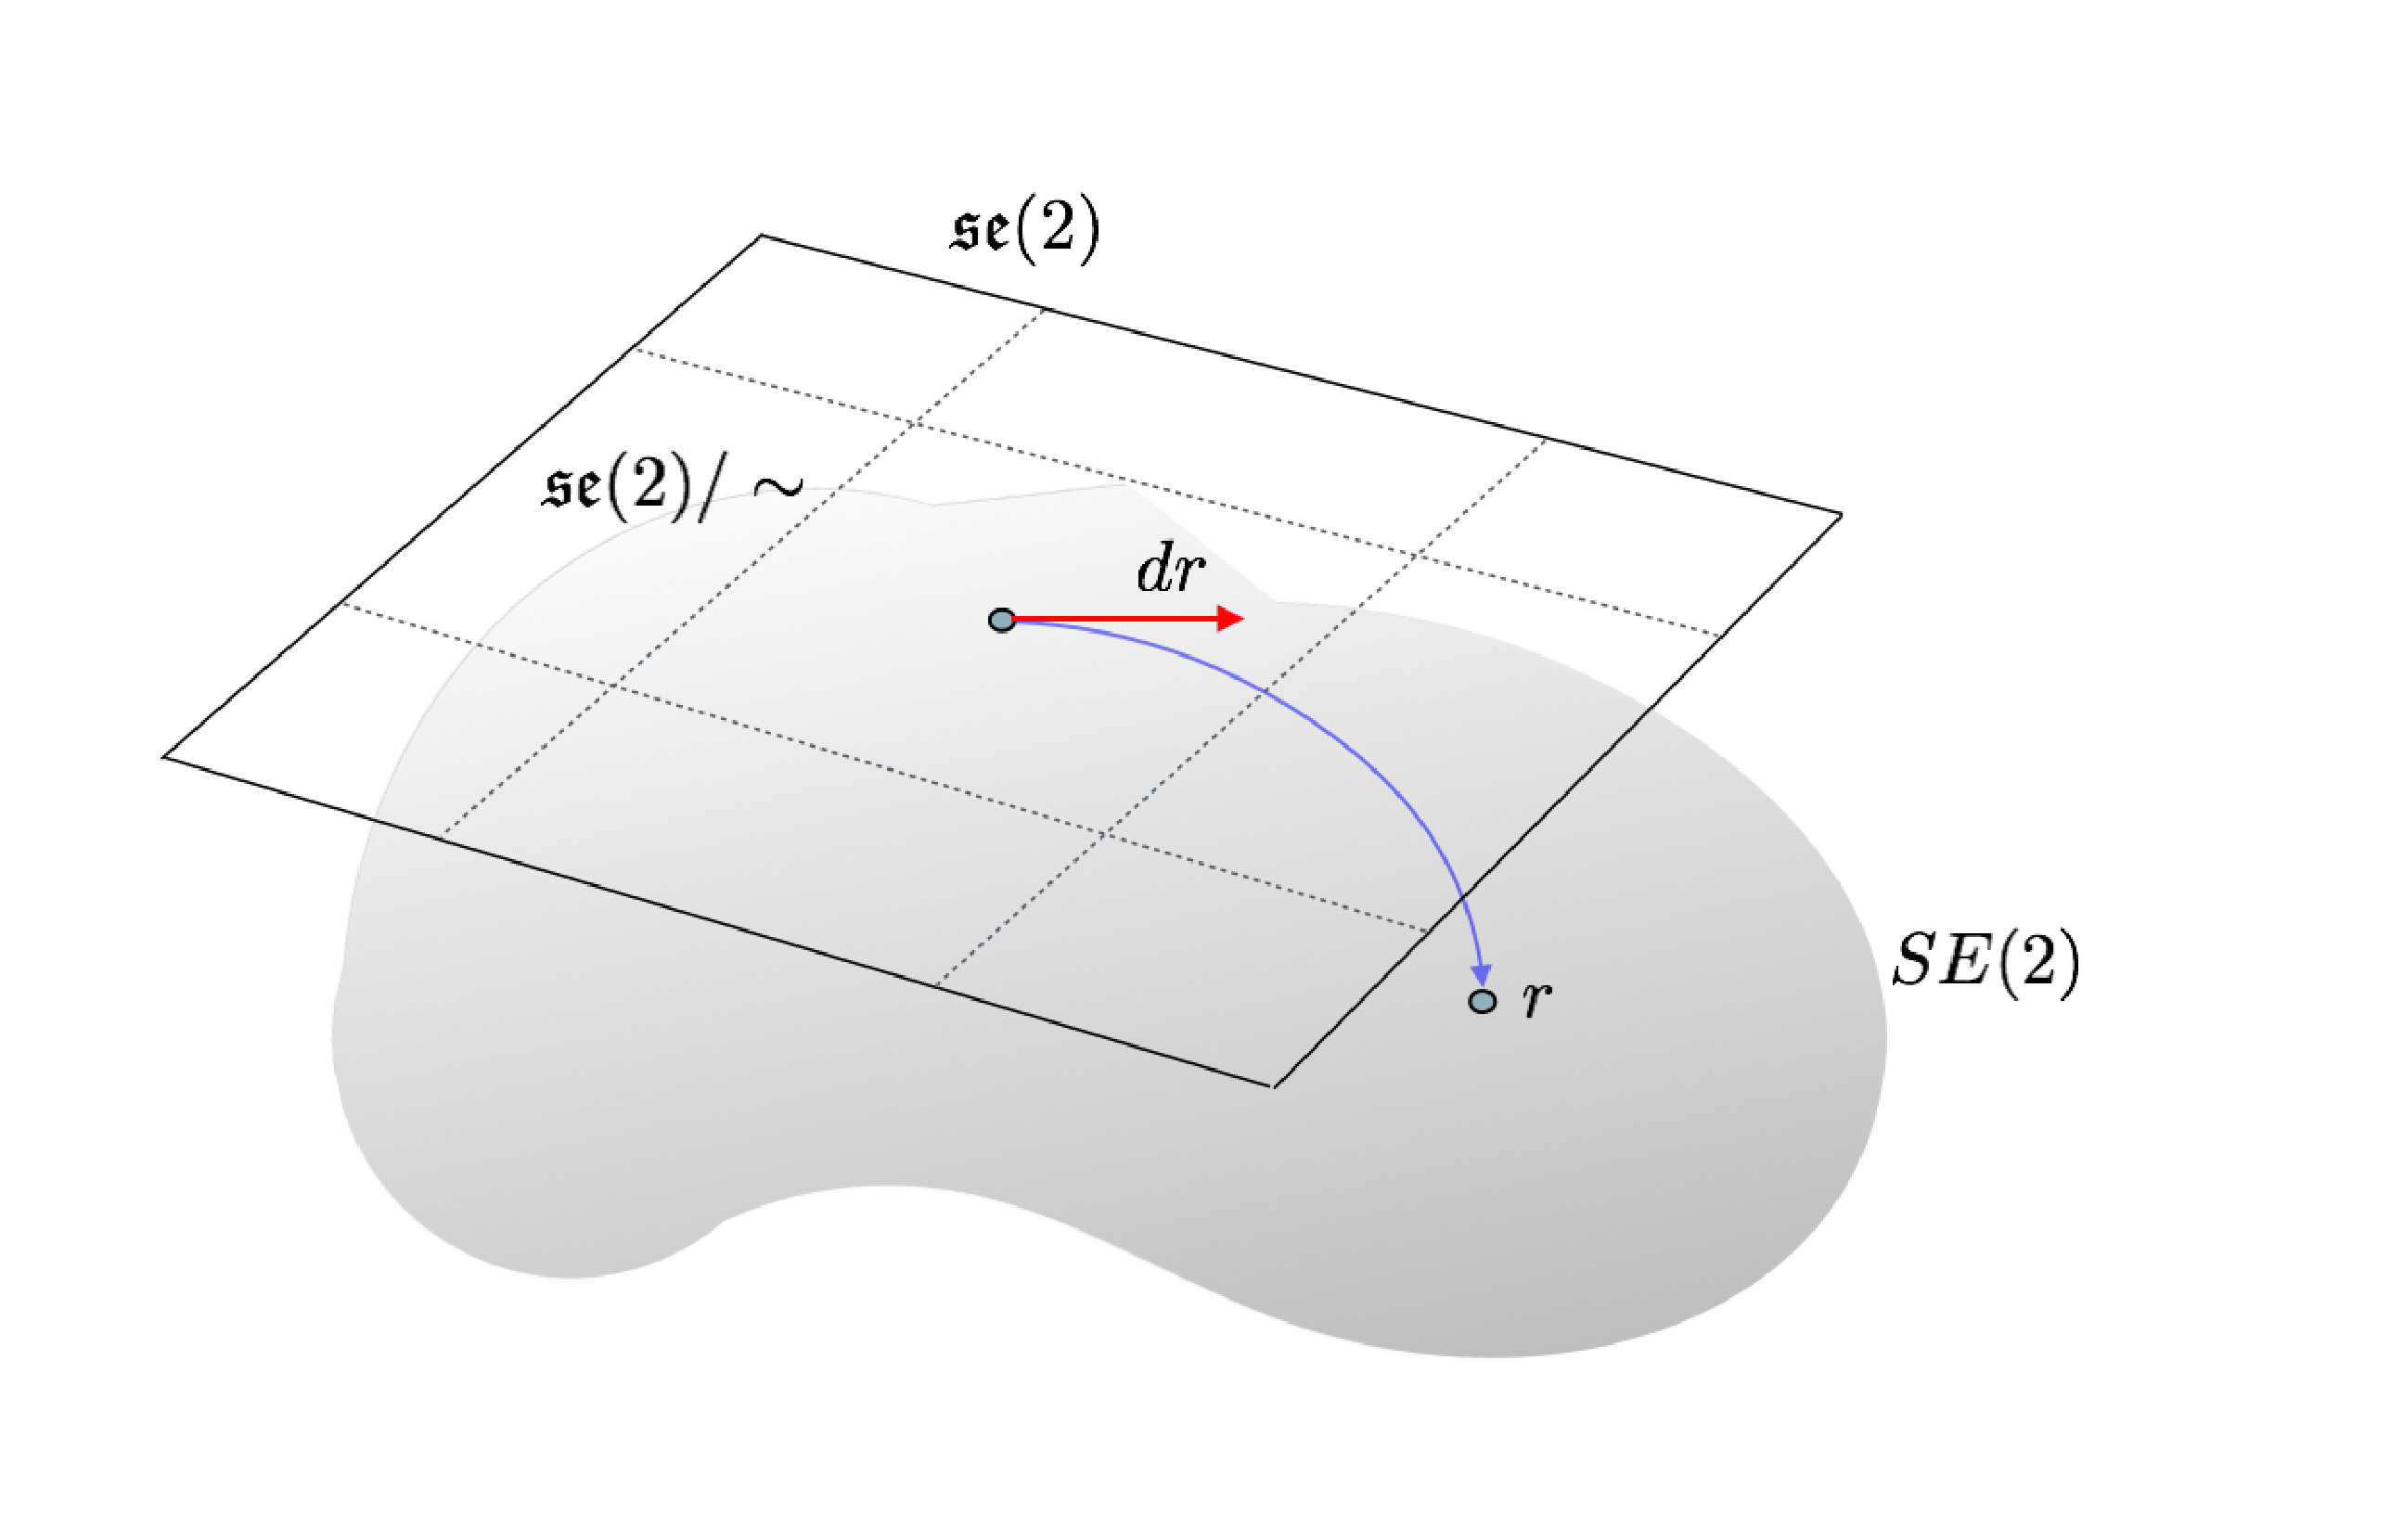
\includegraphics[scale=0.35]{figures/exp_se2.pdf}
		\caption{The Lie algebra $\mathfrak{se}(2)/\sim$ defined as the quotient of the Lie algebra $\mathfrak{se}(2)$ over the equivalence relation $\sim$ is in bijective correspondence with $SE(2)$.}
		\label{fig:exp_se2}
	\end{figure}
	
\end{enumerate}

% % % % % % % % % % % % % % % % % %
% % % % % % % % % % % % % % % % % % %
\subsection{Computations of Log-composition in $\mathfrak{se}(2)$}
The log-composition of two elements $dr_0 = (\theta_0, dt^{x}_0, dt^{y}_0)$ ans $dr_1 = (\theta_1, dt^{x}_1, dt^{y}_1)$ of $ \mathfrak{se}(2)/\sim$ results
\begin{align}\label{eq:log_composition_se2_closed_form}
& dr_0 \oplus dr_1 =  \log(\exp(dr_0)\circ \exp(dr_1)) 
\end{align}
The approximations of the log-composition using truncated BCH formulas are straightforward:
\begin{align*}
dr_0 \oplus dr_1 &\simeq  BCH^{0}(dr_0,dr_1 ) = dr_0 + dr_1  \\
dr_0 \oplus dr_1 &\simeq BCH^{1}(dr_0,dr_1 ) =  dr_0 + dr_1 + \frac{1}{2}[dr_0, dr_1] \\
dr_0 \oplus dr_1 &\simeq BCH^{2}(dr_{0}, dr_{1}) =  dr_0 + dr_1 + \frac{1}{2}[dr_0, dr_1] + \frac{1}{12}([dr_0,[dr_0, dr_1]] + [dr_1,[dr_1, dr_0]] )
\end{align*}

To compute the approximation with the Taylor method, and so to compute the equation \ref{eq:taylor}, we observe that the restricted form of the Lie bracket is given by
\begin{align*}
[dr_0, dr_1] &= (0, dR(\theta_0)dt_1 - dR(\theta_1)dt_0)^T \\
& = (0, -\theta_0 dt^{y}_1 + \theta_1 dt^{y}_0 ,  \theta_0 dt^{x}_1 - \theta_1 dt^{x}_0)^T
\end{align*} 
Therefore, the adjoint operator can be written in matrix form as a dual matrix of $dr$:
\begin{align*}
\text{ad}_{dr} = 
\left (
\begin{array} {c c c}
0            &  0        &      0\\
dt^y       &  0        & - \theta \\
- dt^x   & \theta &  0
\end{array}
\right )
\end{align*} 
In fact, when applied to $dr_1$ it results in the Lie bracket:
\begin{align*}
\text{ad}_{dr_0} dr_1= 
\left (
\begin{array} {c c c}
0            &  0        &      0\\
dt^{y}_0       &  0        & - \theta_0 \\
- dt^{x}_0   & \theta_0 &  0
\end{array}
\right )
\left (
\begin{array} {c }
\theta_1   \\
dt^{x}_1   \\
dt^{y}_1 
\end{array}
\right )
=
\left (
\begin{array} {c }
0  \\
-\theta_0 dt^{y}_1+ \theta_1 dt^{y}_0\\ 
 \theta_0 dt^{x}_1- \theta_1 dt^{x}_0
\end{array}
\right )
\end{align*} 
To compute the Taylor approximation proposed in equation \ref{eq:taylor} of the log composition, indicating $dt^{\star} = (dt^{y}, - dt^{x})$ it can be proved easily by induction that
\begin{align*}
\text{ad}_{dr}^{n} 
= 
\left (
\begin{array} {c c}
0            &  0        \\
dt^{\star}      &  dR(\theta)      
\end{array}
\right )^n
=
\left (
\begin{array} {c c}
0            &  0        \\
dR(\theta)^{n-1}dt^{\star}      &  dR(\theta)^{n}      
\end{array}
\right )
\end{align*}
And so the series involved in the equation $\ref{eq:taylor}$ become
\begin{align*}
\sum_{n=0}^{\infty} \frac{B_{n}}{n!} \text{ad}_{dr}^{ n} 
=
\sum_{n=0}^{\infty} \frac{B_{n}}{n!} \left (
\begin{array} {c c}
0            &  0        \\
dR(\theta)^{n-1}dt^{\star}      &  dR(\theta)^{n}      
\end{array}
\right ) 
\end{align*}
We can split it in two part, the rotational part $dR(\theta)^{n}$ and the translational part $dR(\theta)^{n-1}dt^{\star}$. The rotational part, using the nature of Bernoulli numbers and its generative equation, when $\theta \neq 0$ become
\begin{align*}
\sum_{n=0}^{\infty} \frac{B_{n}}{n!} dR(\theta)^{n}  
&=
I + \frac{1}{2}dR(\theta) + \sum_{n=1}^{\infty}\frac{B_{2n}}{2n!} dR(\theta)^{2n}  \\
&=
I + \frac{1}{2}dR(\theta) + (\sum_{n=1}^{\infty}\frac{B_{2n}}{2n!} (i \theta)^{2n})I  \\
&=
\frac{1}{2}dR(\theta) + (\sum_{n=0}^{\infty}\frac{B_{n}}{n!}(i \theta)^{n} - \frac{1}{2} i\theta) I  \\
&=
\frac{1}{2}dR(\theta) + (\frac{i\theta e^{i\theta}}{e^{i\theta} - 1} - \frac{1}{2} i\theta) I  \\
&=
\frac{1}{2}dR(\theta) +  \frac{\theta /2}{\tan(\theta/2)} I  
\end{align*}
where the equation $dR(\theta)^{2n} =  (i \theta)^{2n}I  $. For the translational part we have
\begin{align*}
\sum_{n=1}^{\infty} \frac{B_{n}}{n!} dR(\theta)^{n-1} dt^{\star} 
&=
dR(\theta)^{-1} \Big(\sum_{n=1}^{\infty}\frac{B_{n}}{n!} dR(\theta)^{n}\Big)dt^{\star} \\
&=
dR(\theta)^{-1}  \Big(\sum_{n=0}^{\infty}\frac{B_{n}}{n!} dR(\theta)^{n} - I \Big)dt^{\star}  \\
&=
dR(\theta)^{-1}  \Big(\sum_{n=0}^{\infty} \frac{1}{2}dR(\theta) +  \frac{\theta /2}{\tan(\theta/2)} I  - I \Big) dt^{\star} \\ 
&=
dR(\theta)^{-1}  \Big(\sum_{n=0}^{\infty} \frac{1}{2}dR(\theta) +  \frac{\theta /2}{\tan(\theta/2)} I  - I \Big)dt^{\star} \\
&=
\Big(\frac{1}{2} I + (\frac{\theta /2}{\tan(\theta/2)} - 1)dR(\theta)^{-1}   \Big) dt^{\star}    \\
\end{align*}
Finally the closed form for the Taylor approximation of the log-composition is \cite{vercauteren2014preprint}:
\begin{align}
dr_{0}\oplus dr_{1}
=
dr_{0}
+
\sum_{n=0}^{\infty} \frac{B_{n}}{n!} \text{ad}_{dr_{0}}^{ n} 
dr_{1}
+
\mathcal{O}(dr_{1}^2)
=
dr_{0}
+
\mathbf{J}(dr_{0}, dr_{1})
dr_{1}
+
\mathcal{O}(dr_{1}^2)
\end{align}
where 
\begin{align*}
\mathbf{J}(dr_{0}, dr_{1})
=
\left (
\begin{array} {c c c}
1            &  0        &      0
\\
-\frac{\theta_0/2 - \tan(\theta_0/2)}{\theta_0\tan(\theta_0/2)}  dt^{x}_0 + \frac{1}{2}dt^{y}_0       
&  \frac{\theta_0 /2}{\tan(\theta_0/2)} 
& - \theta_0/2 
\\
-  \frac{1}{2} dt^{x}_0 -\frac{\theta_0/2 - \tan(\theta_0/2)}{\theta_0\tan(\theta_0/2)} dt^{y}_0       
& \theta_0/2 
&  \frac{\theta_0 /2}{\tan(\theta_0/2)}
\end{array}
\right )
\end{align*}
therefore the corresponding numerical method indicated with the function $\text{Tl}$ as
\begin{align}\label{eq:taylor_se2}
dr_{0}\oplus dr_{1}
\simeq
Tl(dr_{0}, dr_{1})
:=
dr_{0}
+
\mathbf{J}(dr_{0}, dr_{1})
dr_{1}
\end{align}

The approximation of the log-composition using parallel transport is a straightforward application of the equation \ref{eq:parallel_transport}: 
\begin{align}\label{eq:parallel_transport_se2}
dr_{0}\oplus dr_{1}
&\simeq
pt(dr_{0}, dr_{1}) 
:=
dr_{0}
+
\exp\big(\frac{dr_{0}}{2}\big)   
\exp(dr_{1}) 
\exp\big(-\frac{dr_{0}}{2}\big)
-
I
\end{align}
where the composition in the Lie group coincides with the product of matrix in the bigger algebra $GL(3)$ that contains both the Lie group $SE(2)$ and the Lie algebra $\mathfrak{se}(2)$.


% % % % % % % % % % % % % % % % % % % % % % % % % % % % % % % % % % % %
% % % % % % % % % % % % % % % % % % % % % % % % % % % % % % % % % % % %
% % % % % % % % % % % % % % % % % % % % % % % % % % % % % % % % % % % %
% % % % % % % % % % % % % % % % % % % % % % % % % % % % % % % % % % % %
\section{The Lie group of Diffeomorphisms}\label{se:svf}


As previously said in section \ref{se:diffe_util_and_liab}, the passage from the finite to the infinite dimensional case is not free of deceptions. We will investigate in the next two subsections in particular the following facts that happen for matrices:
\begin{enumerate}
	\item $SE(2)$ and $\mathfrak{se}(2)$ are subset of a bigger algebra, where all of the operations are compatible.
	\item Lie logarithm and Lie exponential are local isomorphisms.
\end{enumerate}


% % % % % % % % % % % % % % % % % % % % % % % % % % % % % % % % % % % %
% % % % % % % % % % % % % % % % % % % % % % % % % % % % % % % % % % % %
\subsection{A bigger algebra for the group of Diffeomorphisms}
As well as for any matrix Lie group, both the group $SE(2)$ and the algebra $\mathfrak{se}(2)$ are subset of the same bigger algebra of the matrices with real entries $GL(3,\mathbb{R})$. The product of the algebra coincides with the composition of the group and thanks to the linearity, scalar product is compatible with the product and with the composition.

The importance of the existence of a bigger is not only a theoretical problem: the power series expansions of the exponential and the logarithm \ref{eq:log_as_inf_sum} \ref{eq:exp_as_inf_sum} as well as expressions as \ref{eq:prop_matrix_diff_log} and \ref{eq:prop_matrix_lim} would me meaningless without the possibility of expressing the sum of two elements of a multiplicative group. In addition if the bigger algebra that contains both Lie group and Lie algebra exists, a unique norm in this space can be defined and used to compare elements in both of the subspaces.

In the case of diffeomorphism of $\Omega\subset \mathbb{R}^d$, we can identify a bigger vector space that contains both Lie group and Lie algebra, but it is less straightforward than in the case of matrices, and for this aim it is necessarily to have some definition at hand.

% deformation, homeomorphisms, diffeomorphisms. map V and displacements. Structures. Figure
We define the set of \emph{deformations}, the set of continuous functions from $\Omega$ to $\Omega$ (a strategy to avoid issues on the boundary of $\Omega$ is to consider the deformations over the whole $\mathbb{R}^d$ that are the identity outside $\Omega$; for our purposes we will consider these definitions equivalent). If a deformation is invertible with continuous inverse then it is called \emph{homeomorphism}; the set of homeomorphisms forms a group with the operation of function composition , indicated with $\text{Hom}(\Omega)$. If an homeomorphism is differentiable and has differentiable inverse then it is called \emph{diffeomorphism}. Again the set of diffeomorphisms forms a group, indicated with $\text{Diff}(\Omega)$.

A \emph{velocity vector field} over $\Omega$ is a function that at each point of $\Omega$, associates a vector of $\mathbb{R}^d$; the set of velocity vector fields, indicated with $\mathcal{V}(\Omega)$ forms a vector space, and considering the multiplication with the Jacobian matrix at each point, it forms a non-commutative group:  
\begin{align*}
\mathbf{u}\cdot \mathbf{v} := J_{\mathbf{u}}\mathbf{v}
\qquad
\forall\mathbf{u},\mathbf{v}\in \mathcal{V}(\Omega)
\end{align*}
And thanks to the linearity of the Jacobian, $\mathcal{V}(\Omega)$ forms an algebra.

% here the two doors
There are two ways to associate a velocity vector field to a diffeomorphisms $\varphi$. The first one is subtracting the identity function $1$. If $\mathbf{x}$ is in $\Omega$ and $\varphi(\mathbf{x})$ is the new point after the transformation, then the associated velocity vector field, called here \emph{deformation field of} $\varphi$, is the function that at the point $\mathbf{x}$ associate the vector defined as the difference $\varphi(\mathbf{x}) - \mathbf{x}$. To recover the deformation from a velocity field $\mathbf{u}$ is enough to add the identity; in this case we have the \emph{deformation of} $\mathbf{u}$. We indicate this operation of adding and subtracting the identity with the function $\mathcal{V}$:
\begin{align*}
\mathcal{V}(\varphi) = \varphi - 1 
\qquad \qquad
\mathcal{V}^{-1}(\mathbf{u}) = \mathbf{u} + 1 
\end{align*}
We can see that deformation fields of diffeomorphisms are elements of $\mathcal{V}(\Omega)$, that is the analogous of the bigger algebra that contains Lie group and Lie algebra in the case of matrices.
The second way to associate a velocity vector field to $\varphi$ is with the Lie logarithm defined in the chapter \ref{ch:tools}. It is interesting to notice that when $\mathbf{u}$ is little then $\mathcal{V}^{-1}$ and $\exp$ are closed to each other and $\mathcal{V}^{-1}$ can be considered a good approximation of $\exp$ (see figure \ref{fig:exp_versus_v}). The very same happens for matrices, as noticed in equations \ref{eq:small_rotation_matrices_approx}.

\begin{figure}[!ht]
	\centering
	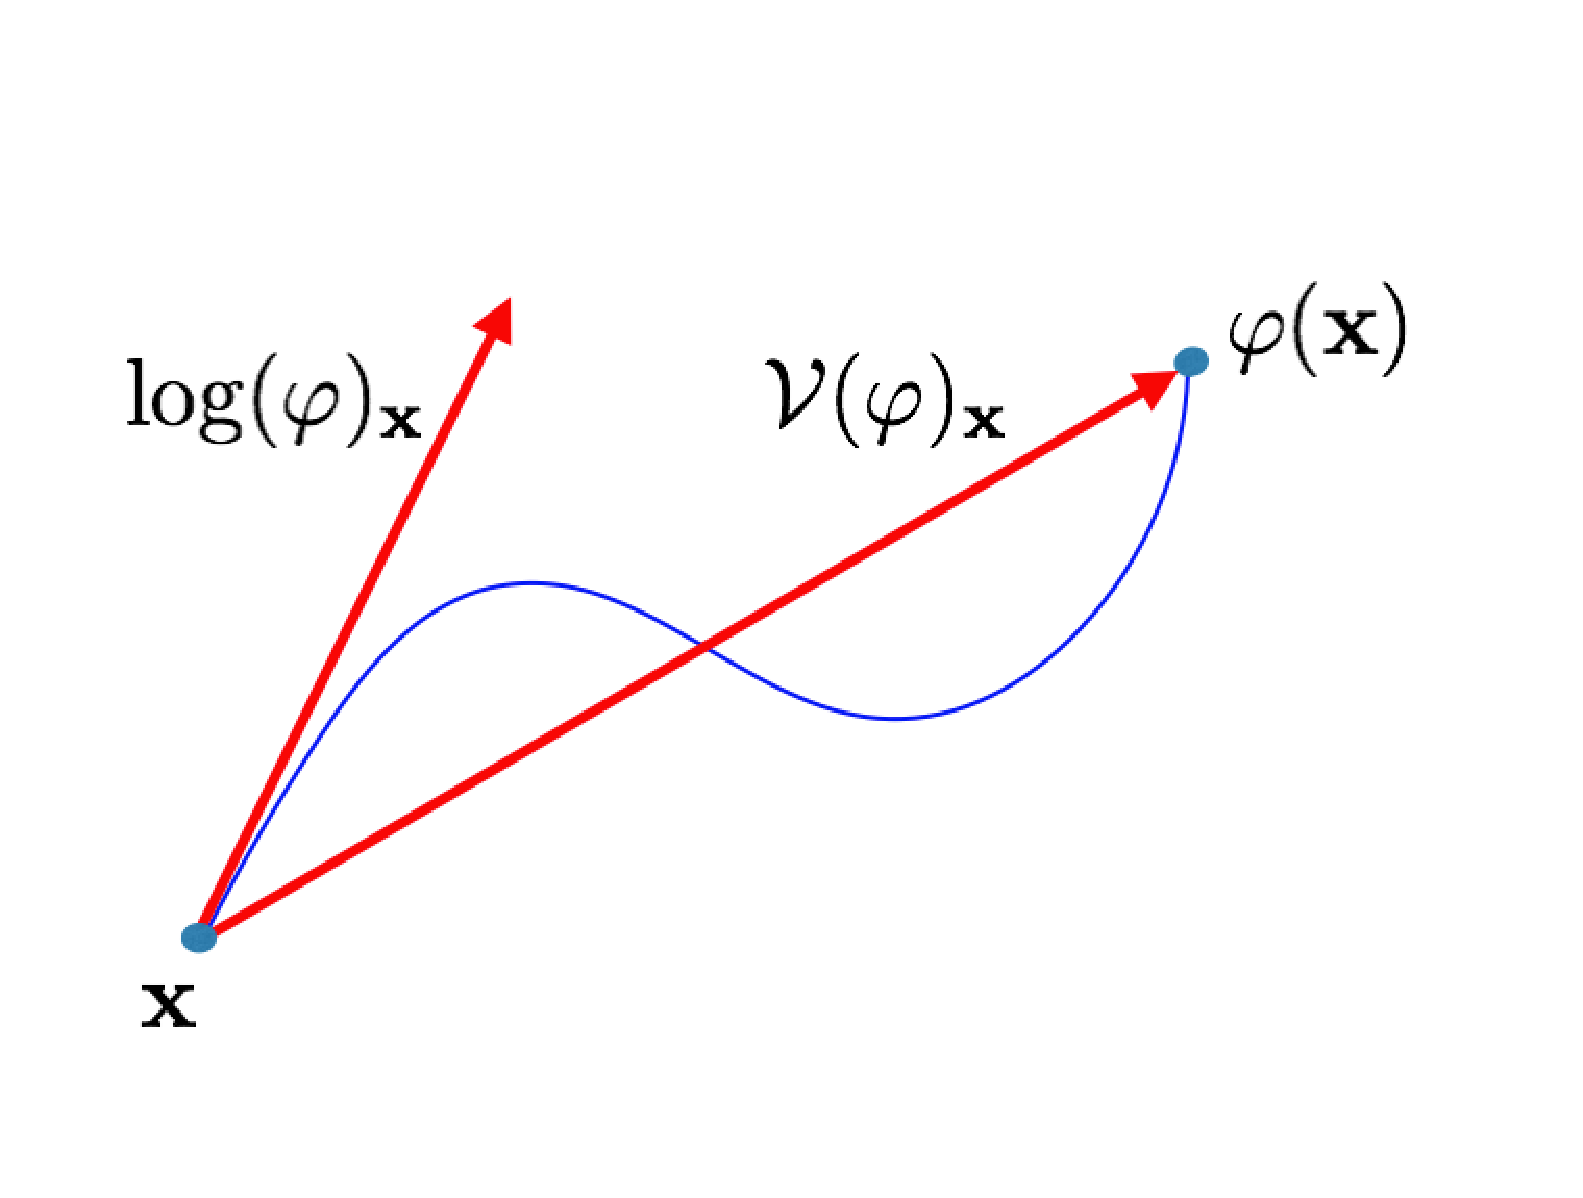
\includegraphics[scale=0.25]{figures/exp_versus_v.pdf}
	\caption{for little deformations, the deformation field $\log(\varphi)$ and the tangent field $\mathcal{V}(\varphi)$ are close to each others.}
	\label{fig:exp_versus_v}
\end{figure}

% difference number 2) exponential map not a local isomorphisms. - cut locus dominio stellato per le matrici. Qualcosa di diverso per i diffeomorfismi
At this point it is important to notice that, while a deformation field of $\varphi$ can always be defined, the exponential map it is not defined for any diffeomorphism. This is the second remarkably difference between the matrix Lie group and the Lie group of diffeomorphisms that will be investigated in the next section.

\subsection{Local isomorphisms for a subset of Diffeomorphisms: one parameter subgroup and stationary velocity fields}

In the case of matrices, the exponential map is a local isomorphisms: it is always possible to find an open neighbor of $\mathbf{0}$ in the Lie algebra and an open neighbor of the identity element in the Lie group (in the same topology induced by the metric inherited by the bigger algebra), such that the exponential map is always defined and invertible.
In the infinite dimensional case there are diffeomorphisms arbitrarily close to the identity that are not embedded to any one-parameter subgroups and therefore can not be related with any element in the tangent space by an ODE (see the counterexample in \cite{lorenzi2013geodesics}, pag. 6 or the definition of Koppel-diffeomorphisms \cite{grabowski1988free} pag. 115).

% subset of diff in which we are interested: the one that can be parmetrized by tangent vector fields
Since for medical image registration we are interested only in the diffeomorphisms that can be parametrized by tangent vector fields, investigate this feature is not only purely a theoretical issue. As happened in the previous section, it is necessarily to have some definitions at hand before moving in this direction. 

% two kinds of vector fields. TVVF SVF. A continuous way to produce diffeomorphims




Approaching the infinite dimensional Lie algebra of diffeomorphisms we can 








%

% Relations between exp(SVF) exp(TVVF) e \Gamma



% % Grid and discretized vector fields 


% % Log computation - Error computation

% % Error computations without any norm.





particular is is always possible to find  the exponentialFor the particular case of diffeomorphisms over the compact subset $\Omega\subset\mathbb{R}^d$, indicated with $\text{\emph{Diff}}(\Omega)$, the exponential map is not a local bijection 

 
We will consider the subset of $\text{\emph{Diff}}(\Omega)$ containing only the diffeomorphisms that are in the image of the exponential function $\exp$. An introduction to this subset is presented in the next section, followed by a section on their parametrization.


% % % % % % % % % % % % % % % % % % % % % % % % % % % % % % % % % % % %
% % % % % % % % % % % % % % % % % % % % % % % % % % % % % % % % % % % %


If we indicate the image of $exp$ as with $\text{\emph{Diff}}^{1}(\Omega)$ of the diffeomorphisms on $\Omega$, then this set represents the diffeomorphisms that belongs to the one-parameter subgroup on the manifold $\text{\emph{Diff}}(\Omega)$.\\
Each of its element are generated by a tangent vector field in $\mathcal{C}^{\infty}(\Omega)$ through an ordinary differential equation (see for example \cite{arnold2006ordinary}). These generating tangent vector field can be divided into two classes, as well as the related ODE:
\begin{enumerate}
	\item Stationary  - or homogeneous
	\begin{align*}
	\frac{d\varphi(t)}{dt} = V_{\varphi(t)}
	\end{align*}
	\item Non-stationary - or non-homogeneous
	\begin{align*}
	\frac{d\varphi(t)}{dt} = V_{(t, \varphi(t))}
	\end{align*}
\end{enumerate}
For a fixed $t$ both the stationary vector field (or SVF) $V_{\varphi(t)}$ and the time varying vector field (or TVVF) $V_{(t, \varphi(t))}$ have solutions that belong to $\text{\emph{Diff}}^{1}(\Omega)$. When varying $t$, the TVVFs behave as continuous paths over the tangent vector field, corresponding to the one-parameter subgroup $\text{\emph{Diff}}^{1}(\Omega)$ through the map $\exp$.\\
Thanks to the Cauchy theorem that ensures the uniqueness of the solution of the ODE under the initial condition $\varphi(0) = e$, the local bijection between $\text{\emph{Diff}}^{1}(\Omega)$ and the Lie algebra of the tangent vector fields over $\Omega$ is ensured (see \cite{milnor1982infinite}, \cite{khesin2008geometry}):
\begin{align*}
\mathcal{V}(\Omega) \simeq  \text{\emph{Diff}}^{1}(\Omega) \subset \text{Diff}(\Omega)
\end{align*}
and, as consequence of the definition of $\exp$ and $\log$ it follows that
\begin{align*}
\text{\emph{Diff}}^{1}(\Omega) &= \exp( \mathcal{V}(\Omega))\\
\mathcal{V}(\Omega) &= \log(\text{\emph{Diff}}^{1}(\Omega))
\end{align*}
In the LDDMM framework (briefly mentioned in section \ref{se:state_of_the_art}) only TVVFs are considered, while after subsequent paper of \cite{arsigny2006log} the attention has been restricted to SVF for practical applications.\\
For our purposes when talking about diffeomorphisms, we will take into account only the one embedded in the one-parameter subgroup $\text{\emph{Diff}}^{1}(\Omega)$ - the image of a SVF through the $\exp$ map - with a particular parametrization, presented in the next section. 

% % % % % % % % % % % % % % % % % %
% % % % % % % % % % % % % % % % % % %
\subsection{Norm for stationary velocity fields}


% % % % % % % % % % % % % % % % % %
% % % % % % % % % % % % % % % % % % %
\subsection{Parametrization of SVF: Grids and Discretized Vector Fields}\label{se:parametrization_SVF}

Even if images are discrete elements, the underpinning model of the transformations is based on the continuous. There are several motivations that led to this choice: as underlined by \cite{szeliski1994image}, the most important is that images are discrete measurement of the continuous property of an object. Therefore it is reasonable have a model as close as possible to the continuous object rather than to a set of discrete measurements. 
Certainly it is important to keep in mind the fact that the continuous approximation is obtained - in a non unique way - from the discretized image with an interpolation scheme. This imply that, for example if the distance between two separate objects is less than the size of a voxel, in continuous approximation based on the discretized image the two object will be not anymore separated.

% discretization 
ggetti e misure con cui si ha a che fare quando si parla di SVF discretizzati. Esempi con immagini. 

As in many other implementation, the data structure utilized to store deformation fields are 5-dimensional matrices
\begin{align}\label{eq:basic_data_structure}
M = M(x_i,y_j,z_k,t,d) \qquad (i,j,k)\in L , ~~ t \in T  ~~ d = 1,2,3
\end{align}
where $(x_i,y_j,z_k)$ are discrete position of a lattice $L$ in the domain of the images, $t$ is the time parameter in a discretized domain $T$ and $d$ is index of the coordinate axis. So, the discretized \emph{tangent vector} $\mathbf{v}_{\tau}(x_i,y_j,z_k)$ at time $t$, has coordinates defined by
\begin{align*}
\mathbf{v}_{t}(x_i,y_j,z_k) = (M(x_i,y_j,z_k,t ,1), M(x_i,y_j,z_k,t,2), M(x_i,y_j,z_k,t ,3))
\end{align*}
% update 
At the $k$-th step, the algorithm provides the 5-dim matrix $\mathbf{v}_{k}$ that is the approximation of the discretized time varying velocity fields $V_{(t,\phi_{t} (\mathbf{x}))}$. The update at each step is computed as
\begin{align*}
\mathbf{v}_{k+1} = \mathbf{v}_{k} - \epsilon \vec{\nabla} (\Delta\mathcal{E})
\end{align*}
where $\Delta\mathcal{E}$ is the discretized version of the energy function and $\epsilon$ is the gradient descent step size.




%Here it may be possible to see the beginning of the problem we have to deal with for the rest of the research, each time passing from the finite dimensional case to the infinite dimensional case.\\
%The domain of the logarithm is the matrix Lie group $\mathbb{G}$ in which only the composition (the matrix product) is defined. Nevertheless it is possible to compute $I + \mathbf{c}$, and this still make sense, and satisfy remarkable properties, when applied to the $\log$. In addition the domain of the exponential is the matrix Lie algebra $\mathfrak{g}$, but the exponential can be nevertheless applied to any matrix, and still be defined.\\
%\emph{This can be done thanks to the fact that for matrices, $\mathfrak{g}$ and $\mathbb{G}$ are subset of a bigger algebra, the algebra of invertible matrices $GL(n)$ \cite{kirillov2008introduction}}. In this structure the operation of sum is still defined over the group that in the general case admits only compositions, and the infinite series \ref{eq:exp_as_inf_sum}, \ref{eq:log_as_inf_sum} are doors to pass from the structure of group to the algebra and vice versa. When presenting the rigid body transformation in chapter \ref{ch:spatial_transformations} we will may open another couple of access doors based on numerical approximations.
%
%When dealing with diffeomorphism in practical applications we have to deal with a theoretical as well as with a practical issue.
%On one side the
%the operations in Lie algebra are not compatible with the composition in the Lie group: expression as $e + \mathbf{v}$ contains a sum that is undefined (and therefore meaningless) in the Lie group structure.
%On the other side 
%the - extremely - continuous nature of diffeomorphisms is not compatible with the - extremely - discrete nature of computers. It is not possible to implement something that maintains any of the property of diffeomorphism in a computer. The only options we have for practical implementations are the vector fields discretized on a $d$ dimensional grid. In the paper of Arsigny \cite{arsigny2006log}, \emph{scaling and squaring} and \emph{inverse scaling and squaring} are proposed for the computation of exponential and logarithm respectively; these algorithms transform a discretized vector field in another discretized vector field, while theoretical domain and codomain of these transformations are radically different. In addition, as shown in \cite{hernandez2008comparing} for some parameters of Stationary LDDMM and the diffeomorphic Demons the diffeomorphisms involved do not preserve the signs of the Jacobian determinant, and therefore are not diffeomorphisms anymore. 
%
%The passage from finite dimensional case of matrices to infinite dimensional case of diffeomorphisms requires a way to represent diffeomorphisms having only discrete vector fields to deal with, where operations within Lie algebra and Lie group are not anymore compatible. The strategy here proposed is to define an operation in the Lie algebra $\mathfrak{g} = \mathcal{V}(\Omega)$ that reflects the properties of the composition in the corresponding Lie group structure $\mathbb{G} = \text{Diff}(\Omega)$.






% % % % % % % % % % % % % % % % % %
% % % % % % % % % % % % % % % % % % %
\subsection{Computations of Log-composition for SVF}\label{se:log_composition_SVF}
A closed-form for the Taylor Expansion method \ref{se:taylor_expansion} to compute the log-composition with elements in $\text{\emph{Diff}}^{1}(\Omega)$ is not known. We will therefore compare the truncated BCH formula with the parallel transport method \ref{se:parallel_transport}. 
The Lie bracket that appears of SVF in the truncated $BCH$ of degree $0,1,1.5$ and $2$, are computed using the Jacobian matrix $J$:
\begin{align}
[\mathbf{u},\mathbf{v}] :=J_{u}\mathbf{v} - J_{u}\mathbf{v}  
\qquad
\forall \mathbf{u},\mathbf{v} \in \mathfrak{g}
\end{align}
as a consequence of its definition (see \cite{lee2012introduction}).
It has been shown that this definition is uniquely defined as action on the space of $\mathbb{C}^{\infty}$ function on the same domain and it satisfies the axioms of Lie bracket of a Lie algebra.\\

Therefore the truncated approximation of the BCH formula presented in the equation \ref{eq:bch_definition} become:
\begin{align*}
BCH^{0}(\mathbf{u},\mathbf{v}) &= \mathbf{u} + \mathbf{v} \\
BCH^{1}(\mathbf{u},\mathbf{v}) &=  \mathbf{u} + \mathbf{v} + \frac{1}{2}(J_{\mathbf{u}}\mathbf{v} - J_{\mathbf{u}}\mathbf{v})\\
BCH^{3/2}(\mathbf{u},\mathbf{v}) 
&=  
\mathbf{u} + \mathbf{v} + \frac{1}{2}(J_{u}\mathbf{v} - J_{u}\mathbf{v}) + 
\frac{1}{12}\big( 
2 J_{\mathbf{u}} J_{\mathbf{u}}\mathbf{v} +2 J_{\mathbf{u}} J_{\mathbf{v}}\mathbf{u}
- 
J_{(J_{\mathbf{u}}\mathbf{v} - J_{\mathbf{u}}\mathbf{v})}\mathbf{u} 
\big) 
\\
BCH^{2}(\mathbf{u},\mathbf{v}) 
&=  
\mathbf{u} + \mathbf{v} + \frac{1}{2}(J_{u}\mathbf{v} - J_{u}\mathbf{v}) 
\\
&+ 
\frac{1}{12}\big( 
2 J_{\mathbf{u}} J_{\mathbf{u}}\mathbf{v} +2 J_{\mathbf{u}} J_{\mathbf{v}}\mathbf{u}
- 
J_{(J_{\mathbf{u}}\mathbf{v} - J_{\mathbf{u}}\mathbf{v})}\mathbf{u} 
+
2 J_{\mathbf{v}} J_{\mathbf{v}}\mathbf{u} +2 J_{\mathbf{v}} J_{\mathbf{u}}\mathbf{v}
- 
J_{(J_{\mathbf{v}}\mathbf{u} - J_{\mathbf{v}}\mathbf{u})}\mathbf{v} 
\big) 
\end{align*}
Lie brackets of SVF can become extremely small, in particular, as we will see in the last chapter, when the standard deviation of the Gaussian filter that generates the fields is small. \\
Whether it is not known how to apply Taylor method presented in \ref{se:taylor_expansion} for the SVF, the parallel transport method for the computation of the log-composition follows directly from equation  \ref{eq:parallel_transport}:
\begin{align*}
\mathbf{u}_0\oplus \mathbf{u}_1
&\simeq
\mathbf{u}_0 
+
\exp_{e}\big(\frac{\mathbf{u}_0}{2}\big)   
\circ  \exp_{e}(\mathbf{u}_1) 
\circ \exp_{e}\big(-\frac{\mathbf{u}_0}{2}\big)
-
e
\end{align*}
Here the exponential function can be computed with several algorithms (scaling and squaring, forward Euler, composition method, Taylor expansion, see \cite{bossa2008algorithms} for a comparison of their performances). Following the original setting of the Log-euclidean metric proposed in \cite{arsigny2006log} we use the scaling and squaring, keeping in mind that this choice impact on the results.








